\section{Overview of \lancet}\label{sec:overview}



\begin{figure}[tb]
\centering
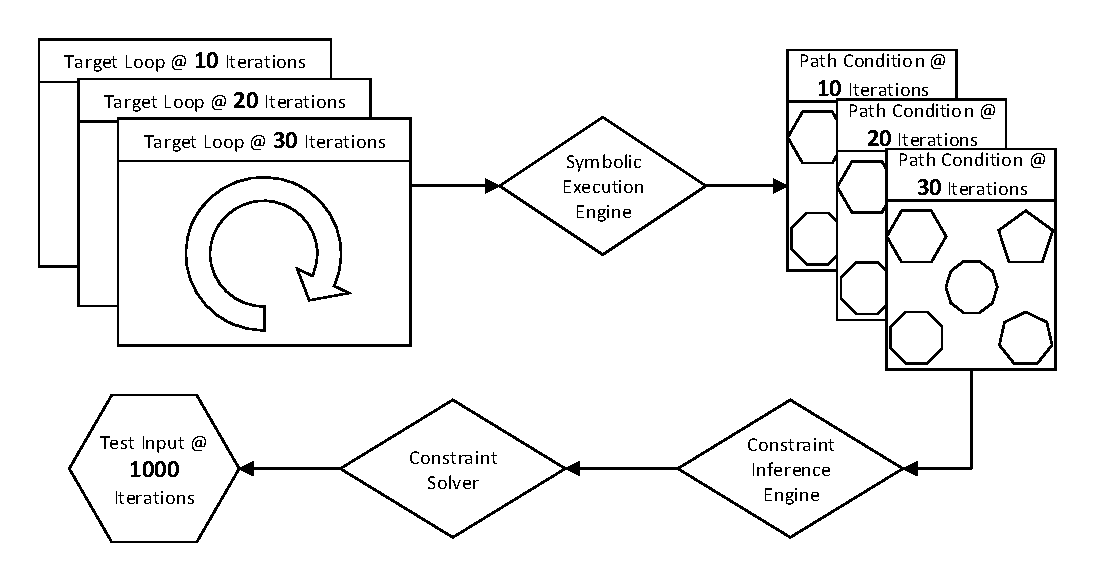
\includegraphics[width=\linewidth]{figures/method}
\caption{High level flow of \lancet's approach for generating inputs to run a loop 1000 times.}
\label{fig:method}
\end{figure}

Figure~\ref{fig:overview} shows the basic operation of \lancet. After the target loop in the program is identified (Section~\ref{sec:target-loop}), \lancet generates a set of path constraints that satisfy a {\em loop-iteration meta-constraint} that the target loop executes exactly $k$ times. For small $k$, this is done by augmenting KLEE~\cite{klee} with a custom {\em loop-centric} path-exploration heuristic (Section~\ref{sec:loop-centric}). 

While traditional dynamic symbolic execution techniques suffice to generate path constraints that run a loop a small number of times, they are impractical for large $k$: running a loop thousands of times will require orders of magnitude more invocations to \lancet's constraint solver than running a loop tens of times, and will be unacceptably slow. \lancet's novel approach to this problem is to determine the path constraints that satisfy the loop-iteration meta-constraint for a large $k$ {\em without performing symbolic execution}.

To achieve this goal, \lancet takes the following steps. First, \lancet generates a {\em series} of path constraint sets, each for different small values of $k$. It then analyzes those path constraints to separate the constraints in those sets into {\em validity constraints}---constraints that ensure that inputs are well-formed---and {\em scaling constraints}---constraints that determine how many times the target loop runs (Section~\ref{sec:validity-constraints}). \lancet then uses the scaling constraints to train a statistical model that relates the value of $k$ to the associated scaling constraints, and uses this model to {\em infer what the scaling constraints would look like} for large $k$ (Section~\ref{sec:constraint-inference}). These inferred scaling constraints are then perturbed slightly to account for modeling error and combined with the validity constraints to produce a new constraint set, which can be solved with a constraint solver, generating a large-scale input for the program (Section~\ref{sec:input-generation}). Crucially, once the initial training phase of \lancet is complete, inputs that target {\em any scale} can be generated at the same overhead (though potentially different levels of accuracy), making \lancet a truly scalable approach to generating large-scale, stress-test inputs.

% The search for a path of a given number of iterations of the target loop begins with executing the program with an arbitrary input, e.g. an existing hand-crafted test case, trying to discover as many new paths as possible with a search strategy that is a mix of random walk and code coverage heuristics, until any of the paths it explored enters the target loop. From there on, \lancet switches to a loop-centric search strategy which prioritizes the paths that keep iterating the loop over those that exit. The path searching process continues until \lancet finds a path that has reached the requested trip count.
